% !TeX root = ../tfg.tex
% !TeX encoding = utf8

\chapter{Planteamiento del problema} \label{chap:planteamiento-problema}

\section{Fundamentos de la tomografía computarizada}
La tomografía computarizada es una técnica médica esencial que permite obtener imágenes no invasivas del interior del cuerpo humano sin la superposición de distintas estructuras anatómicas, a diferencia de la fluoroscopia de rayos X planar \parencite{buzug2011computed}. Originalmente, la TC, introducida clínicamente en 1971, solo permitía obtener imágenes axiales del cerebro, pero ha evolucionado para producir imágenes tridimensionales de cualquier área anatómica \parencite{calzado2010tomografia}.

La radiografía convencional produce proyecciones bidimensionales de un objeto tridimensional, lo que conlleva una reducción de la información espacial y una disminución del contraste debido al promedio de las estructuras. La TC fue el primer método en superar este problema, logrando un alto contraste que permite incluso la visualización de tejidos blandos.

Las aplicaciones médicas de la TC se centran principalmente en la imagenología tridimensional. El primer paso es adquirir un conjunto de rebanadas bidimensionales, lo que se conoce como reconstrucción secundaria. Esto se logra moviendo al paciente ligeramente en la dirección axial del escáner (eje z). 

Una vez que se tiene un volumen de datos, se pueden generar diferentes vistas:

\begin{itemize}
    \item \textbf{Reformateo Multiplanar (MPR)}: permite mostrar secciones anguladas a través del conjunto de rebanadas tridimensional. Los planos anatómicos principales que se presentan a los radiólogos son las rebanadas axiales, sagitales y coronales \ref{fig:ct_ejes_anatomicos}. 
    \item \textbf{Renderizado de Volumen (Volume Rendering)}: esta técnica asigna valores físicos de reflexión y dispersión de luz a cada voxel (píxel espacial), simulando una iluminación virtual para crear una imagen óptica artificial del volumen.
    \item \textbf{Renderizado de Superficie (Surface Rendering)}: en esta técnica, se selecciona un umbral de valor de gris para representar una superficie, que luego se aproxima mediante triángulos y se ilumina virtualmente.
    \item \textbf{Endoscopia virtual}: se pueden producir vistas interiores de órganos huecos y vías respiratorias.
\end{itemize}

La resolución espacial en el plano coronal mejora considerablemente al disminuir el grosor de corte reconstruido, tanto en la representación volumétrica como en las imágenes coronales.

\begin{figure}[!htbp]
    \centering
    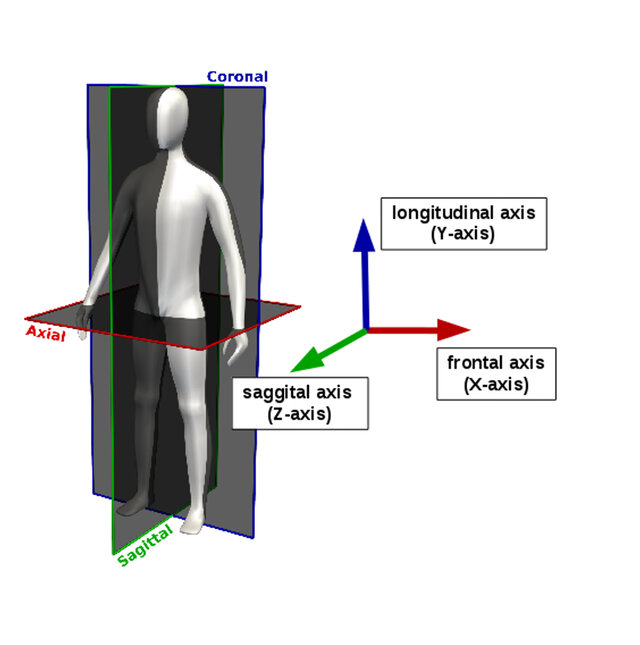
\includegraphics[width=0.7\textwidth]{img/ejes_ct.jpg}
    \caption{Visualización de los planos anatómicos estándar con el sistema de coordenadas correspondiente. Se distinguen tres planos de vista estándar: axial (vista superior), sagital (vista lateral) y coronal (vista frontal). La anatomía se define mediante los siguientes ejes anatómicos: frontal (eje X), longitudinal (eje Y) y sagital (eje Z). Fuente: \cite{heim2018large}}
    \label{fig:ct_ejes_anatomicos}
\end{figure}


En resumen, la TC funciona utilizando rayos X y algoritmos especiales para reconstruir imágenes del interior del cuerpo. A partir de múltiples proyecciones bidimensionales tomadas desde diferentes ángulos, se generan imágenes tridimensionales que permiten ver con detalle la anatomía interna. Estas imágenes pueden visualizarse en cortes axiales, sagitales o coronales, o incluso con técnicas de renderizado más avanzadas que ayudan al diagnóstico médico de forma más precisa.

\section{Descripción general del problema}
La biopsia pulmonar guiada por TC es un procedimiento diagnóstico fundamental para caracterizar lesiones pulmonares y confirmar la presencia de cáncer. Es un paso crucial en el diagnóstico que puede tener un impacto significativo en el resultado para el paciente: 
\begin{itemize}
    \item \textbf{Diagnóstico temprano y mejora de la supervivencia}: el cáncer de pulmón es la causa principal de mortalidad por cáncer y su tasa de supervivencia a 5 años es solo del 18\%, en gran parte debido al diagnóstico en etapas avanzadas \parencite{deng2018clinical}. Por lo tanto, el diagnóstico temprano mediante biopsia es fundamental para mejorar la supervivencia a largo plazo.
    \item \textbf{Confirmación y caracterización}: la biopsia permite obtener muestras de tejido o células para confirmar la presencia de cáncer y determinar sus características específicas, lo cual es esencial para la planificación del tratamiento. Los enfoques para la biopsia de lesiones pulmonares se han desarrollado para proporcionar métodos convenientes y precisos para este diagnóstico.
    \item \textbf{Adaptabilidad a la ubicación de la lesión}: existen diversas técnicas de biopsia que se seleccionan considerando la ubicación y la situación de las lesiones. 
\end{itemize} 

Aunque las biopsias son cruciales para el diagnóstico del cáncer de pulmón, conllevan ciertos riesgos o complicaciones, cuya incidencia puede variar según la técnica utilizada y las características de la lesión. 

En una revisión sistemática de la literatura médica existente realizada por \cite{deng2018clinical}, se encontró con los siguientes resultados tras una biopsia pulmonar transtorácica con aguja guiada por TC (CT-guided PTNB): las dos complicaciones más frecuentes son el neumotórax (acumulación de aire entre el pulmón y la pared torácica) y la hemorragia. Se reportó una incidencia de neumotórax del 22.69\% (946 de 4170 casos) y de hemorragia del 7.08\% (138 de 1949 casos). 
La precisión diagnóstica y la incidencia de complicaciones pueden verse afectadas por el tamaño de la lesión (lesiones más pequeñas pueden disminuir la precisión y aumentar las complicaciones) o la longitud del trayecto de la aguja (trayectos más largos pueden aumentar las complicaciones).


\section{Interés del problema: aplicaciones en medicina}

El interés real de predecir el riesgo de complicaciones en biopsias pulmonares radica en mejorar la seguridad y la calidad del proceso diagnóstico del cáncer de pulmón. Un número considerable de neoplasias pulmonares requiere confirmación histológica mediante biopsia, a menudo guiada por TC. Aunque se trata de un procedimiento generalmente seguro, no está exento de complicaciones relevantes, siendo el neumotórax y la hemorragia pulmonar las más frecuentes.

Actualmente, la estimación del riesgo previo a la biopsia depende en gran medida de la experiencia del médico y de factores clínicos generales como la edad, el historial del paciente o el tamaño y la localización de la lesión. Sin embargo, estos criterios resultan limitados y no permiten una evaluación cuantitativa y personalizada del riesgo. No existen herramientas clínicas que ofrezcan una predicción fiable y objetiva antes de la realización del procedimiento, lo que deja un margen importante para la mejora.

En este contexto, surge la oportunidad de aplicar técnicas de inteligencia artificial y deep learning para desarrollar un sistema predictivo capaz de anticipar complicaciones antes de la biopsia. Este enfoque innovador permitiría abordar el problema como una tarea de clasificación binaria: predecir si un paciente desarrollará complicaciones o no, a partir de datos clínicos tabulares e imágenes médicas tridimensionales. La IA puede detectar patrones sutiles en las características radiómicas de las imágenes, como la textura o la densidad del tejido, imperceptibles para el ojo humano pero potencialmente asociados a un mayor riesgo de complicación.

El desarrollo de una herramienta de este tipo tendría aplicaciones clínicas directas y muy relevantes. Podría integrarse en los sistemas de visualización radiológica para ofrecer al especialista una estimación cuantitativa del riesgo al seleccionar la lesión de interés. Esto facilitaría una toma de decisiones más informada, permitiendo:

\begin{itemize}
    \item Identificar a los pacientes con mayor riesgo de complicaciones.
    \item Adaptar la técnica de biopsia o planificar precauciones adicionales.
    \item Optimizar los recursos sanitarios, por ejemplo, planificando disponibilidad de sangre o material específico si se anticipa un riesgo elevado de hemorragia.
    \item Plantear estrategias diagnósticas alternativas en casos seleccionados.
\end{itemize}

En última instancia, esta herramienta contribuiría a reducir la incidencia de efectos adversos y mejorar la seguridad del paciente, permitiendo además personalizar el procedimiento en función de factores de riesgo conocidos como la presencia de enfisema pulmonar, lesiones de pequeño tamaño o muy próximas a la pleura, o signos radiológicos de hipertensión pulmonar.

En particular, cabe destacar que actualmente no existen investigaciones o literatura científica que aborden de forma específica la predicción del riesgo de complicaciones en biopsias pulmonares mediante técnicas de inteligencia artificial. Esta falta de estudios previos subraya el carácter novedoso de este problema y añade un reto significativo al desarrollo del proyecto. Implica la necesidad de explorar enfoques metodológicos sin referentes establecidos, diseñar estrategias de preprocesamiento y modelado desde cero, y validar cuidadosamente la utilidad clínica de los modelos desarrollados. Este vacío en la investigación hace que la presente propuesta no solo sea innovadora, sino también especialmente relevante para abrir nuevas líneas de trabajo en la aplicación de la IA al apoyo a la decisión médica en procedimientos invasivos.



\section{Descripción de los datos}
La base de datos utilizada en este estudio está formada por un total de 125 pacientes, recopilados de forma progresiva gracias a la colaboración con el Hospital Universitario Clínico San Cecilio de Granada. El primer lote de datos se recibió el 6 de diciembre de 2024, con información de 30 pacientes. A partir de entonces, se fueron incorporando nuevos casos aproximadamente entre dos semanas y un mes, hasta alcanzar los 125 pacientes el 1 de julio. Para cada paciente se dispone de una TC, que constituye un volumen tridimensional. En la mayoría de los casos, estos estudios están centrados en la región pulmonar, aunque algunos incluyen exploraciones de cuerpo entero.
La base de datos se encuentra totalmente anonimizada, cumpliendo con todas las normativas de privacidad y protección de datos personales. 

Los volúmenes 3D presentan variabilidad en sus dimensiones y en el número de cortes o slices ya que el propio hospital tiene diferentes máquinas para hacer las TC. Aunque se ha realizado un preprocesado para ajustar ciertas características, existe heterogeneidad en cuanto al tamaño original de las imágenes, lo cual se gestiona en la fase de preprocesamiento mediante técnicas de normalización y ajuste de tamaño para homogenizar los datos de entrada. En la Figura \ref{fig:ejemplos_planos256x512-label} tenemos un ejemplo de un volúmen desde los tres planos anatómicos. 

Las características de los volúmenes son las siguientes:
\begin{itemize}
    \item \textbf{Número de datos}: 125 pacientes.
    \item \textbf{Tamaño de los datos}: (768,768,x) o (512,512,x) donde la x es el número de slices que varía en cada volumen. 
    \item \textbf{Formato original}: DICOM.
\end{itemize}


\begin{figure}[!htbp]
    \centering
    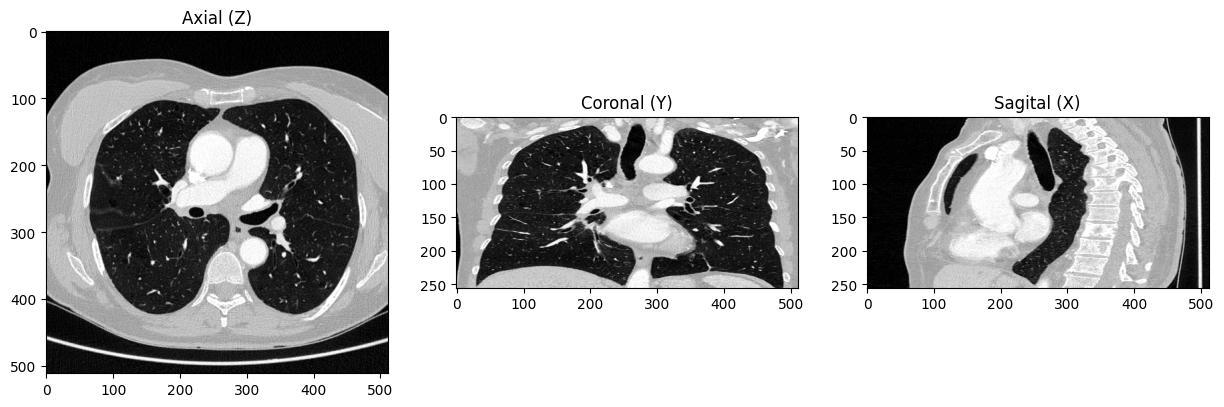
\includegraphics[width=1\textwidth]{img/ejemplos_planos256x512.png}
    \caption{Visualización de un volumen 3D de tamaños (256,512,512) desde los tres planos anatómicos: axial, coronal y sagital. Elaboración propia.}
    \label{fig:ejemplos_planos256x512-label}
\end{figure}

A parte de los volúmenes 3D, disponemos un fichero de datos con datos clínicos tabulares sobre los pacientes. Estos datos incluyen características demográficas, factores de riesgo, información sobre el diagnóstico y evolución de la enfermedad, así como detalles de mutaciones genéticas. La estructura de los datos tabulares es la siguiente: 
\begin{itemize}
    \item \textbf{Paciente}: Identificador anónimo del paciente.
    \item \textbf{Sexo y Edad}: Información demográfica del paciente.
    \item \textbf{Tipo de Cáncer}: Clasificación del tumor pulmonar.
    \item \textbf{Complicación}: Indicación de si el paciente presentó alguna complicación relacionada.
    \item \textbf{Tipo de Complicación}: Especificación de la complicación, en caso de existir.
    \item \textbf{Factor de Riesgo}: Hábitos o condiciones previas del paciente que pueden influir en el diagnóstico (tabaquismo, alcoholismo, obesidad, HTA, DM...).
    \item \textbf{Patología Pulmonar}: Presencia de otras patologías pulmonares adicionales (enfisema paraseptal, enfisema centrolobulillar, fibrosis, neumonía...).
    \item \textbf{Extensión al Diagnóstico}: Evaluación inicial de la extensión del cáncer.
    \item \textbf{TC}: Tipo de dispositivo utilizado para la adquisición de las imágenes de tomografía (Philips B, GE Optima, Philips I, Siemens S...). 
    \item \textbf{Extensión a los 5 años}: Información sobre la progresión del cáncer a largo plazo.
    \item \textbf{Mutación}: Presencia de mutaciones genéticas relevantes en el diagnóstico (p40, p63, CK5/6, CK7...).
\end{itemize}

De todas estas características solo vamos a utilizar las que conocemos antes de hacer la biopsia. Estas variables son: sexo, edad, factor de riesgo y patología pulmonar. Todas las demás características las sabemos una vez realizada la biopsia, por lo que no sirven para la inferencia. La etiqueta a predecir será complicación si estamos ante clasificación binaria o bien tipo de complicación si estamos ante clasificación multietiqueta, ya que se pueden dar varias complicaciones a la vez en un mismo paciente. 

El identificador del paciente es una codificación de los datos más relevantes del mismo:

\begin{itemize}
    \item \textbf{Número de dato:} entero.
    \item \textbf{Sexo:} Mujer (M) u Hombre (H).
    \item \textbf{Tipo de cáncer:} Adenocarcinoma (A), Epidermoide (E), Linfoma de Hodgkin (H), No tumor: posible TBC (T), Linfoma T (L)...
    \item \textbf{Complicación:} Sí o No.
    \item \textbf{Tipo de complicación:} X si no hay complicación y, en caso contrario, se especifica (Hemorragia leve, Neumotórax, Leve derrame pleural...).
\end{itemize}

Por ejemplo, el identificador \textit{1MASh} indica que es el primer paciente de la base de datos, es mujer, tiene adenocarcinoma y ha tenido complicación la cual es hemorragia.

Estos datos clínicos y de imagen se integrarán en el proceso de preprocesamiento y modelado para extraer características relevantes y realizar predicciones diagnósticas. En la siguiente sección se detallarán las transformaciones y selecciones aplicadas sobre esta información para su uso en modelos de aprendizaje automático y profundo.

\subsection{Formato de los datos}
A lo largo de toda esta investigación, se han utilizado diferentes formatos de datos para almacenar y procesar la información. Los volúmenes originales estaban en formato DICOM, que es el estándar para imágenes médicas, y se han convertido a NIfTI para facilitar su manipulación en entornos de análisis de datos. Además, se han utilizado archivos en formato npy para entrenar los modelos.

\paragraph{DICOM}
El formato DICOM (Digital Imaging and Communication in Medicine) se desarrolló para facilitar el intercambio de manera independiente del fabricante del equipo. Además de almacenar las propias imágenes, DICOM  \texttt{.dcm} incluye metadatos relevantes que describen cada estudio, lo que mejora la organización y la interpretación de la información. Gracias a ello, permite un intercambio de datos rápido y seguro, evitando confusiones y errores que podrían surgir al gestionar múltiples archivos para un mismo estudio \parencite{mustra2008overview}.

No solo es un formato de archivo, sino también un protocolo de comunicación de red. Es decir, un archivo DICOM, además de soportar los datos de la imagen, también contiene otra información útil para describirla. Esta información adicional (metadatos), como la descripción del objeto, datos del paciente, procedimientos realizados o informes, y detalles técnicos del dispositivo de imagen (p. ej., fabricante, número de serie, tiempo de exposición para mamografía), se almacena en un encabezado (header). El encabezado DICOM es muy completo, específico de la modalidad y auto-descriptivo, lo que permite que el software entienda cómo se produjo la imagen  \parencite{larobina2014medical}. En nuestro proyecto vienen anonimizados, por lo que esta información viene vacía y no nos da ventaja. 


\paragraph{NIfTI}
NIfTI (Neuroimaging Informatics Technology Initiative) es un formato de archivo desarrollado a principios de la década de 2000 con el objetivo de facilitar y reforzar el análisis de post-procesamiento, especialmente en neuroimagen \parencite{larobina2014medical}.

Típicamente, las imágenes NIfTI  \texttt{.nii} se guardan como un único archivo .nii que fusiona el encabezado (metadatos) y los datos de píxeles \parencite{singh2023secure}.

Además, admite una amplia gama de tipos de datos, incluyendo enteros (con y sin signo, de 8 a 64 bits), flotantes (de 32 a 128 bits) y complejos (de 64 a 256 bits), lo que minimiza la necesidad de factores de escala.

\paragraph{npy}
El formato \texttt{.npy} es el formato nativo de NumPy para almacenar arrays multidimensionales de forma eficiente. En este proyecto se ha utilizado para guardar los volúmenes ya preprocesados como matrices NumPy, listos para ser cargados directamente durante el entrenamiento de los modelos. Este formato ofrece ventajas en términos de velocidad de lectura y escritura, simplicidad de estructura (al contener únicamente datos binarios y metainformación mínima sobre el array) y compatibilidad directa con los pipelines de procesamiento en Python. 

En conclusión, de los formatos descritos, DICOM es el estándar más ampliamente utilizado en entornos clínicos. Se le considera el principal formato de todos los departamentos de imágenes médicas y el estándar líder adoptado por los principales proveedores de equipos de diagnóstico. NIfTI, por su parte, es el formato por defecto en la investigación de neuroimagen y se usa para el intercambio de datos de CT \parencite{larobina2014medical}.


\subsection{Legalidad de los datos}
Los datos médicos utilizados en este proyecto corresponden a volúmenes de TC en formato DICOM que han sido previamente anonimizados realizado por el equipo clínico responsable, eliminando todos los identificadores personales directos e indirectos presentes en los metadatos de los archivos DICOM, conforme a las directrices establecidas en el \emph{Considerando 26 del Reglamento (UE) 2016/679 (RGPD)} \parencite{gdprRecital26}, que estipula que los datos anonimizados de manera irreversible quedan fuera del ámbito de aplicación del RGPD.

En consecuencia, y de acuerdo con lo establecido en la \emph{Ley Orgánica 3/2018}, de \emph{Protección de Datos Personales y garantía de los derechos digitales}, concretamente en su \emph{Disposición adicional decimoséptima, apartado 2, letra e} \parencite{lopd2018}, se considera que no existe ninguna probabilidad razonable de reidentificación de los sujetos a partir de los datos empleados en este estudio. De este modo, se garantiza el pleno cumplimiento de la normativa vigente en materia de protección de datos personales, en línea con las recomendaciones y criterios establecidos por la \emph{Agencia Española de Protección de Datos (AEPD)} \parencite{aepdAnonimizacion}.

Esta garantía de anonimización y cumplimiento normativo es esencial para el desarrollo responsable de proyectos de IA en el ámbito médico, asegurando la protección de la privacidad de los pacientes y el respeto a sus derechos fundamentales.


\section{Dificultades del problema}
El problema de la predicción de complicaciones en biopsias pulmonares mediante inteligencia artificial y técnicas de radiómica representa un desafío considerable en el ámbito de la investigación médica. A diferencia de otras aplicaciones de la IA en medicina, donde se han realizado progresos significativos en la predicción de diagnóstico y clasificación de tumores, la predicción de riesgos asociados a procedimientos invasivos, como la biopsia pulmonar, es un campo aún inexplorado. Actualmente, no existe literatura científica relevante que aborde este problema de forma directa, lo cual evidencia la novedad y la dificultad de esta línea de investigación. Esta falta de estudios previos dificulta la identificación de enfoques metodológicos exitosos y obliga a explorar múltiples técnicas y configuraciones para evaluar su efectividad. Además, la falta de referencias previas introduce un grado de incertidumbre adicional, ya que ni siquiera se tiene la certeza de que esta línea de trabajo sea abordable; es decir, no se sabe si los datos presentan indicios suficientes para identificar patrones y poder predecir los riesgos de manera fiable y precisa.

Una de las principales dificultades encontradas es la disponibilidad de datos. En el ámbito clínico, los datos son limitados y su obtención depende del ritmo de trabajo en los centros hospitalarios. En este trabajo, la recopilación de nuestros datos se realiza exclusivamente en el Hospital Universitario Clínico San Cecilio. De Internet solo se han utilizado datasets para realizar el preentrenamiento en tareas similares, ya que no existen bases de datos públicas con etiquetas específicas de complicaciones en biopsias pulmonares por ser un tema de investigación nuevo en la literatura. Esta restricción impone un límite al volumen de datos disponibles, lo cual dificulta el entrenamiento de modelos de machine learning robustos. Además, los datos tienden a estar desbalanceados, ya que las complicaciones graves son eventos poco frecuentes. Este desbalance entre clases introduce dificultades adicionales en el proceso de entrenamiento, dado que los algoritmos tienden a sobreajustarse a la clase mayoritaria, perdiendo capacidad de generalización para detectar correctamente los eventos adversos.

Adicionalmente, la complejidad del problema se incrementa debido a la naturaleza del propio procedimiento. A diferencia de la detección de tumores en imágenes, donde se buscan anomalías estructurales evidentes, la predicción de complicaciones implica identificar patrones sutiles en la textura, densidad y estructura del tejido pulmonar que puedan estar relacionados con un mayor riesgo. Estos patrones no siempre son evidentes y su detección precisa requiere modelos complejos y técnicas avanzadas de extracción de características.

Por último, cabe destacar el reto de la interpretabilidad. En el ámbito médico, la capacidad de explicar las decisiones tomadas por un modelo predictivo es fundamental para su aceptación clínica. Sin embargo, los modelos de deep learning, que son los que han demostrado mayor capacidad predictiva en tareas relacionadas con imágenes, suelen actuar como cajas negras, dificultando la justificación de sus predicciones. Esta falta de interpretabilidad añade una barrera más en la adopción de estas tecnologías para la toma de decisiones clínicas. 

\section{Metodología}

La metodología de trabajo se enmarca en un enfoque empírico orientado a resolver un problema aplicado en la intersección de la ingeniería informática y la medicina. Se han empleado herramientas y técnicas de deep learning para procesar y analizar volúmenes de TC con el objetivo de predecir complicaciones asociadas a biopsias pulmonares, trabajando con datos reales anonimizados cedidos por el Hospital Universitario Clínico San Cecilio de Granada.

Además, el desarrollo de este trabajo se ha realizado siguiendo un método de trabajo estructurado e inspirado en el método científico, adaptado al problema de predicción del riesgo de complicaciones en biopsias pulmonares mediante técnicas de deep learning:

\begin{itemize}
    \item \textbf{Observación.} Estudio del estado del arte en predicción de complicaciones médicas y en el uso de modelos de deep learning para análisis de imagen médica, especialmente en tomografía computarizada pulmonar. Identificación de la ausencia de estudios específicos para predecir el riesgo en biopsias pulmonares, y análisis de la importancia clínica de este problema.
    
    \item \textbf{Formulación de hipótesis.} Planteamiento de la hipótesis de que es posible predecir el riesgo de complicaciones en biopsias pulmonares a partir de datos clínicos tabulares y volúmenes 3D de TC procesados, empleando modelos de deep learning y aprendizaje automático clásico.
    
    \item \textbf{Recogida de datos.} Recolección progresiva de datos anonimizados en colaboración con el Hospital Universitario Clínico San Cecilio de Granada, incluyendo volúmenes DICOM de TC y variables clínicas asociadas a cada paciente. 
    
    \item \textbf{Preprocesamiento y segmentación.} Diseño de pipelines de preprocesamiento avanzados para normalizar intensidades, ajustar tamaños volumétricos y generar representaciones multiventana. Implementación de segmentación automática del pulmón para restringir el área de análisis del modelo a la región anatómicamente relevante.
    
    \item \textbf{Prueba de hipótesis.} Entrenamiento de modelos de deep learning sobre los datos preprocesados, comparando distintos enfoques (con y sin segmentación, diferentes arquitecturas y configuraciones) para evaluar la capacidad predictiva sobre el riesgo de complicaciones.
    
    \item \textbf{Comprobación y análisis.} Evaluación de los resultados obtenidos mediante métricas específicas de clasificación, matrices de confusión, y comparación con expectativas clínicas. Identificación de limitaciones, discusión de resultados y valoración del potencial clínico real del modelo.
    
    \item \textbf{Conclusiones.} Extracción de conclusiones sobre la viabilidad del enfoque propuesto, la importancia de un preprocesamiento cuidadoso (especialmente la segmentación pulmonar), y la necesidad de futuras líneas de investigación para validar y mejorar los resultados en entornos clínicos reales.
\end{itemize}


\subsection{Software}
El desarrollo del código se ha realizado en \texttt{Python 3.12.7}, un lenguaje flexible y ampliamente utilizado en Inteligencia Artificial \parencite{python}. Para la implementación de los modelos de deep learning se ha empleado \texttt{PyTorch 2.5.1}, una librería de código abierto que facilita el trabajo con redes neuronales y permite el uso eficiente de GPUs  (\emph{Graphics Processing Units}, unidades de procesamiento de gráficos) para acelerar las operaciones sobre tensores \parencite{paszke2019pytorch}.

En el proyecto también ha sido utilizado \texttt{MONAI} (Medical Open Network for Artificial Intelligence), concretamente la versión 1.4.0, un framework basado en PyTorch especializado en imagen médica \parencite{cardoso2022monai}. MONAI ha permitido diseñar pipelines de preprocesamiento avanzados y consistentes para volúmenes 3D, incluyendo transformaciones personalizadas como \texttt{Windowingd} y \texttt{MultiWindowingd} para la normalización de intensidades en unidades Hounsfield, así como técnicas de data augmentation en 3D con \texttt{RandAffined}. Se definieron diferentes pipelines para entrenamiento y validación, integrando resize trilineal a un tamaño fijo, normalización, generación de canales multiventana y conversiones a tensores. También se implementaron transformaciones para combinar máscaras segmentadas con las imágenes de entrada, utilizando estrategias como enmascarado o apilado de canales.

Además, se desarrolló un módulo de segmentación automática basado en la herramienta \texttt{TotalSegmentator}, que permitió generar de forma sistemática las máscaras pulmonares a partir de volúmenes TC originales \parencite{wasserthal2023totalsegmentator}. Este paso fue clave para restringir la atención del modelo únicamente al pulmón, evitando que aprendiera correlaciones insignificantes de regiones fuera del área de interés clínico. El script de segmentación automatiza la conversión de lotes de archivos NIfTI en máscaras segmentadas, con soporte para ejecución en GPU o CPU.

Se han diseñado utilidades específicas para el particionado del dataset, permitiendo la generación de splits de entrenamiento, validación y test de forma reproducible y estratificada. Esto incluyó soporte para divisiones simples y k-fold cross-validation, asegurando el equilibrio de clases en cada partición. Todo el sistema de organización de datos se estructuró para mantener trazabilidad y facilitar la reutilización en distintos experimentos.

Para el manejo de datos médicos se utilizó \texttt{NiBabel} (lectura y escritura de archivos NIfTI) \parencite{nibabel}, \texttt{NumPy} para operaciones matriciales \parencite{harris2020array} y \texttt{Matplotlib} para visualizaciones 2D y 3D de imágenes \parencite{Hunter:2007}, segmentaciones y resultados intermedios del preprocesamiento. Para el manejo de tablas y datos clínicos tabulares se empleó \texttt{Pandas} \parencite{mckinney-proc-scipy-2010}, y para la extracción de características radiómicas a partir de volúmenes médicos se utilizó la librería \texttt{PyRadiomics} \parencite{van2017computational}. La fase de desarrollo y pruebas se realizó utilizando \texttt{Visual Studio Code} como editor principal \parencite{vscode}, junto con \texttt{Jupyter Notebooks} para análisis exploratorio, transformaciones y visualización interactiva de resultados \parencite{jupyter}. También han sido utilizadas las librerías \texttt{scikit-learn 1.5.2} \parencite{scikit-learn} y \texttt{scikit-image 0.25.0} para otras utilidades \parencite{van2014scikit}.

Además, en todo momento se ha utilizado el programa \texttt{3D Slicer} para controlar la visualización, procesamiento, segmentación y análisis de los volúmenes 3D \parencite{pieper20043d}. 

Todo el código desarrollado se encuentra disponible en el siguiente repositorio de GitHub: \url{https://github.com/mcribi/TFG}.

\subsection{Hardware}

En cuanto al hardware, el desarrollo inicial se realizó en un portátil personal Victus by HP Gaming Laptop 16-r0xxx las siguientes especificaciones: 

\begin{itemize}
    \item \textbf{Procesador (CPU)}: 13th Gen Intel® Core™ i7-13620H a 4.9 GHz.
    \item \textbf{Memoria RAM}: 32 GB.
\end{itemize}

Para las tareas de entrenamiento y evaluación de modelos se emplearon los servidores de cómputo de alto rendimiento (NGPU) proporcionados por la Universidad de Granada (UGR) cuyas máquinas se encuentran ubicadas en CPD Santa Lucía. 

La infraestructura NGPU de la UGR cuenta con un clúster de nodos de cómputo que incluyen diversas configuraciones de GPUs como GTX Titan, X Pascal, GTX Titan Xp, RTX 2080 Ti, Titan RTX, Tesla V100 (32GB) y Tesla A100 (40GB). Estas han permitido entrenar tanto modelos 2D como 3D.


\section{Técnicas para abordar el problema}
A continuación se describen de forma general todas las técnicas y estrategias empleadas a lo largo del proyecto, que se explican en mayor detalle en las distintas secciones de esta memoria.

En primer lugar, se realizó un análisis exploratorio de datos (EDA) exhaustivo, que incluyó la \textit{visualización de gráficas} y el \textit{análisis estadístico} de variables tanto clínicas como de imagen. Este paso fue clave para comprender la distribución de los datos, identificar posibles sesgos y diseñar las estrategias de preprocesamiento más adecuadas.

El preprocesamiento de los datos jugó un papel esencial. En el caso de las imágenes médicas en TC, se aplicaron \textit{ventanas de Hounsfield} para normalizar intensidades en rangos clínicamente relevantes, y se incorporó un paso de \textit{segmentación pulmonar} mediante la herramienta TotalSegmentator, con el objetivo de centrar el análisis exclusivamente en el pulmón. También se realizaron procesos de \textit{limpieza de ortografía} y unificación en las variables clínicas, \textit{eliminación de columnas irrelevantes}, \textit{normalización} de variables numéricas y \textit{binarización} de variables multietiqueta. Para los volúmenes 3D se implementaron \textit{transformaciones} como el \textit{windowing multicanal} y la \textit{interpolación trilineal} para ajustar los datos a diferentes tamaños estándar ((256,512,512), (128,256,256), (64,64,64), (28,28,28), (128,128,128)), permitiendo así su uso en redes convolucionales con diferentes capacidades y restricciones de memoria. Además, se aplicaron técnicas de \textit{data augmentation} para mejorar la capacidad de generalización de los modelos.

En el caso de los modelos 2D, se utilizaron arquitecturas basadas en \textit{EfficientNetV2-S} con pesos preentrenados en ImageNet1\_v1, aplicando técnicas de \textit{fine-tuning} con congelación de capas. El entrenamiento incluyó \textit{validación cruzada} (5-fold simple, 5-fold estratificada, 5-fold estratificada por paciente) y enfoques \textit{leave-one-out}. Para mejorar el entrenamiento se incorporaron técnicas como el \textit{EarlyStopping} y se empleó la función de pérdida binaria (\textit{BCE Loss}).

Para los modelos 3D se trabajó principalmente con \textit{DenseNet121} y \textit{ResNet} adaptados a volúmenes tridimensionales. Se exploraron diferentes funciones de pérdida como \textit{CrossEntropyLoss} (incluyendo variantes ponderadas con \textit{class weights} calculados según la distribución de clases) y \textit{Focal Loss} para abordar el desbalanceo. También se empleó el \textit{WeightedRandomSampler} con distintos exponente de ponderación para ajustar la probabilidad de muestreo de las clases minoritarias. Se trató el desbalanceo ya que, aunque en el total de datos recogidos no hay un gran desbalanceo, en fechas anteriores sí existía un gran desbalanceo hacia la no complicación. El optimizador principal fue \textit{AdamW}, acompañado del scheduler \textit{ReduceLROnPlateau} para el ajuste dinámico del learning rate y otros programas. Para mitigar el problema de memoria (out of memory) al trabajar con volúmenes grandes y batch sizes pequeños, se implementó \textit{acumulación de gradiente} para simular batch sizes mayores. Asimismo, se aplicaron técnicas de data augmentation específicas para la clase minoritaria mediante transformaciones como \textit{RandFlip}, \textit{RandRotate90d}, \textit{RandZoomd} y \textit{RandGaussianNoise}. El entrenamiento se complementó con técnicas de explicabilidad como \textit{Grad-CAM}, tanto en 2D como en 3D, para analizar la atención del modelo y validar su interpretabilidad clínica.

También se exploró el uso de un \textit{dataset genérico} de CT pulmonar disponible públicamente, con el objetivo de evaluar la viabilidad del problema y la capacidad de los modelos para predecir el tipo de cáncer. Este conjunto de datos se preprocesó de forma equivalente y se entrenó con modelos 3D (DenseNet121), aplicando técnicas de explicabilidad y funciones de pérdida adaptadas al fuerte desbalanceo entre clases. 

Finalmente, se aplicaron técnicas de \textit{aprendizaje automático clásico} sobre los datos tabulares y sobre \textit{características radiómicas} extraídas de las imágenes mediante \textit{PyRadiomics}, entrenando modelos con distintos hiperparámetros y aplicando estrategias de balanceo como SMOTE para mitigar el desequilibrio de clases.



\section{Presupuesto}

A continuación, se presenta el presupuesto estimado para la realización del proyecto \textit{Predicción de Complicaciones en Biopsias Pulmonares mediante Inteligencia Artificial}. Este presupuesto incluye los recursos humanos necesarios para el desarrollo del proyecto, la capacidad de cómputo para el entrenamiento y validación de los modelos predictivos, así como otros servicios adicionales requeridos. La duración total del proyecto se estima en \textit{8 meses}, de diciembre del 2024 a julio del 2025. 

Se excluyen de este presupuesto los costes personales propios del investigador, como el uso de un ordenador portátil, el alquiler de vivienda o el consumo eléctrico doméstico.

Las fuentes para la estimación de costes son \textit{Glassdoor} \footnote{\url{https://www.glassdoor.es/Sueldos/junior-software-engineer-sueldo-SRCH_KO0\%2C24.htm}}, \textit{SalaryExpert} \footnote{\url{https://www.salaryexpert.com/salary}} y \textit{Google Cloud} \footnote{\url{https://cloud.google.com/compute/gpus-pricing}} respectivamente.

\subsection{Recursos Humanos}

El equipo del proyecto está compuesto por el investigador principal (responsable del desarrollo y análisis de modelos de predicción), un médico colaborador (encargado de la validación clínica y supervisión médica de los datos) y el tutor académico que supervisa el trabajo. A continuación, en la Tabla \ref{tab:recursos-humanos}, se detallan los costes asociados.

\begin{table}[!htbp]
    \centering
    \begin{tabular}{|l|c|c|c|}
        \hline
        \textbf{Recurso} & \textbf{Coste Mensual (€)} & \textbf{Duración (meses)} & \textbf{Coste Total (€)} \\ \hline
        Investigador Principal & 1.300 € & 8 & 10.400 € \\ 
        Médico Colaborador    & 2.000 € & 8 & 16.000 € \\ 
        Tutor Académico (25 h) & 2.000 € & 1 & 2.000 € \\ \hline
        \textbf{Total Recursos Humanos} & & & \textbf{28.400 €} \\ \hline
    \end{tabular}
    \caption{Presupuesto destinado a recursos humanos.}
    \label{tab:recursos-humanos}
\end{table}

\subsection{Capacidad de Cómputo}

El desarrollo del modelo predictivo requiere infraestructura de alto rendimiento para procesar imágenes 3D y entrenar redes neuronales. Para ello, se estima el uso de servidores en la nube con GPUs y almacenamiento en la Tabla \ref{tab:computo}.

\begin{table}[!htbp]
    \centering
    \begin{tabular}{|l|c|c|c|}
        \hline
        \textbf{Recurso} & \textbf{Coste Mensual (€)} & \textbf{Duración (meses)} & \textbf{Coste Total (€)} \\ \hline
        Servidores Cloud (GPUs - AWS, GCP) & 100 € & 8 & 800 € \\ 
        Almacenamiento (1 TB en Cloud) & 50 € & 8 & 400 € \\ \hline
        \textbf{Total Capacidad de Cómputo} & & & \textbf{1.200 €} \\ \hline
    \end{tabular}
    \caption{Presupuesto destinado a capacidad de cómputo.}
    \label{tab:computo}
\end{table}

\subsection{Materiales y Otros Gastos}

Para este proyecto no se prevén gastos en licencias de software, ya que todas las herramientas utilizadas son de código abierto y licencia libre (PyTorch, MONAI, PyRadiomics, etc.). Tampoco se consideran necesarias otras compras de materiales o servicios adicionales.

\subsection{Presupuesto Total Estimado}

El presupuesto total estimado para el desarrollo del proyecto durante un periodo de 8 meses asciende a \textbf{29.600 €}, e incluye todos los recursos humanos y la capacidad de cómputo necesarios para su correcta ejecución.


\section{Diario de trabajo}

El desarrollo de este proyecto se ha realizado de forma progresiva a lo largo de varios meses, en estrecha coordinación con el Hospital Universitario Clínico San Cecilio de Granada. Los datos fueron llegando de forma escalonada en distintas entregas, lo que obligó a diseñar un flujo de trabajo adaptable y un preprocesamiento escalable que pudiera incorporar la nueva información conforme se recibía. Las fechas de entrega de los datos fueron las siguientes:

\begin{itemize}
    \item 6 de diciembre de 2024: 30 pacientes.
    \item 30 de enero de 2025: 40 pacientes.
    \item 26 de febrero de 2025: 53 pacientes.
    \item 18 de marzo de 2025: 72 pacientes.
    \item 23 de abril de 2025: 76 pacientes, junto con 100 controles sanos adicionales.
    \item 12 de mayo de 2025: 92 pacientes.
    \item 28 de mayo de 2025: 101 pacientes.
    \item 18 de junio de 2025: 112 pacientes.
    \item 1 de julio de 2025: 125 pacientes en total.
\end{itemize}

Desde diciembre hasta enero incluido, se dedicó tiempo a la revisión de literatura médica relevante para comprender mejor el problema clínico y las variables recogidas por el hospital. Durante este período también se exploraron los programas médicos utilizados y se consolidaron conocimientos de programación en Python aplicados a datos médicos, para sentar las bases del preprocesamiento y análisis posterior.

En febrero, tras este estudio preliminar, se realizó un análisis exhaustivo de las variables tabulares, identificando aquellas relevantes para el entrenamiento y descartando las que no aportaban valor o podían inducir fuga de información. Se desarrolló un análisis exploratorio de datos (EDA) inicial y se comenzó a construir el pipeline de preprocesamiento, con especial atención a su escalabilidad dado que los datos continuarían llegando por lotes. Fue necesario verificar cuidadosamente los datos tabulares e imágenes, ya que se detectaron archivos corruptos que el equipo médico tuvo que reemplazar. Durante esta fase se mantuvieron reuniones con el personal médico para entender de forma cualitativa qué factores clínicos consideran ellos que predicen el riesgo de complicación.

En marzo se experimentó con modelos basados en cortes axiales 2D debido a sus menores requisitos computacionales, pero pronto se comprobó que dividir los volúmenes en slices individuales implicaba una pérdida de información espacial importante. Por ello, se decidió enfocar el desarrollo en modelos 3D completos, ajustando el preprocesamiento tanto para datos 2D como para volúmenes 3D.

Durante abril se trabajó intensamente en abordar el desbalanceo de clases, ya que los datos acumulados hasta esa fecha presentaban una clara predominancia de pacientes sin complicaciones. En este periodo se entrenaron modelos sin segmentación pulmonar, observándose resultados insatisfactorios: las técnicas de explicabilidad mostraban que el modelo se fijaba en regiones ajenas al pulmón. También se probó el preentrenamiento en un dataset público para la predicción del tipo de cáncer pulmonar, pero no se obtuvieron mejoras significativas.

En mayo se incorporó la segmentación pulmonar al pipeline de preprocesamiento, utilizando máscaras generadas con TotalSegmentator para limitar la atención del modelo a la región anatómica relevante. Esta estrategia permitió mejorar los resultados obtenidos. Además, se realizaron los últimos experimentos con modelos 3D, incluyendo nuevas pruebas de preentrenamiento con otro dataset. 

En junio se dedicó por completo a la extracción de características de radiómica y su experimentación.

Finalmente, el mes de julio se dedicó íntegramente a completar y revisar la memoria del trabajo, asegurando la correcta redacción, coherencia y presentación de todos los resultados y conclusiones obtenidas.

Todas estas tareas se pueden agrupar en las siguientes fases:

\begin{itemize}
    \item \textbf{Revisión de la literatura y formación técnica:} estudio de artículos médicos sobre biopsias pulmonares y complicaciones asociadas, revisión de factores de riesgo clínicos y tecnologías de radiómica. Formación en programación en Python aplicada al procesamiento de datos médicos, incluyendo librerías específicas para imágenes 3D.

    \item \textbf{Análisis exploratorio y preprocesamiento:} incluye el análisis y limpieza de datos clínicos, selección de variables relevantes, y exploración de la distribución de las variables y su relación con las complicaciones (EDA). Desarrollo de un diseño modular y escalable para el preprocesamiento, validación manual para corregir errores como archivos corruptos, y generación de máscaras pulmonares con TotalSegmentator para limitar la atención del modelo a la región anatómica relevante.

    \item \textbf{Diseñar modelos:} diseño conceptual del flujo de trabajo de los modelos, definición de la arquitectura base y de las estrategias de integración multimodal (volúmenes TC con datos clínicos), así como consideración de diferentes estrategias para abordar el desbalanceo de clases mediante samplers ponderados o funciones de pérdida adaptadas.

    \item \textbf{Experimentación:} incluye pruebas iniciales con cortes axiales 2D y la posterior transición a modelos 3D completos para preservar la información espacial. Al final, se experimentó con la radiómica. 

    \item \textbf{Fundamentos matemáticos:} estudio de las bases matemáticas para la parte práctica. 

    \item \textbf{Memoria:} redacción progresiva y estructurada de la memoria del TFG a lo largo del proyecto, asegurando la coherencia global, la correcta integración de resultados y el análisis crítico de los mismos.
\end{itemize}


En conjunto, este enfoque permitió mantener una metodología de trabajo estructurada pero flexible, adaptándose a la llegada progresiva de nuevos datos y a los hallazgos intermedios. Además, facilitó la integración de la parte clínica con la informática, asegurando que el resultado final respondiera a una necesidad médica real con una solución técnica sólida y justificada.

Para visualizar el trabajo realizado en estos meses, se muestra un diagrama de Gantt de la planificación en la Figura \ref{fig:gantt_chart}.

\begin{figure}[!htbp]
    \centering
    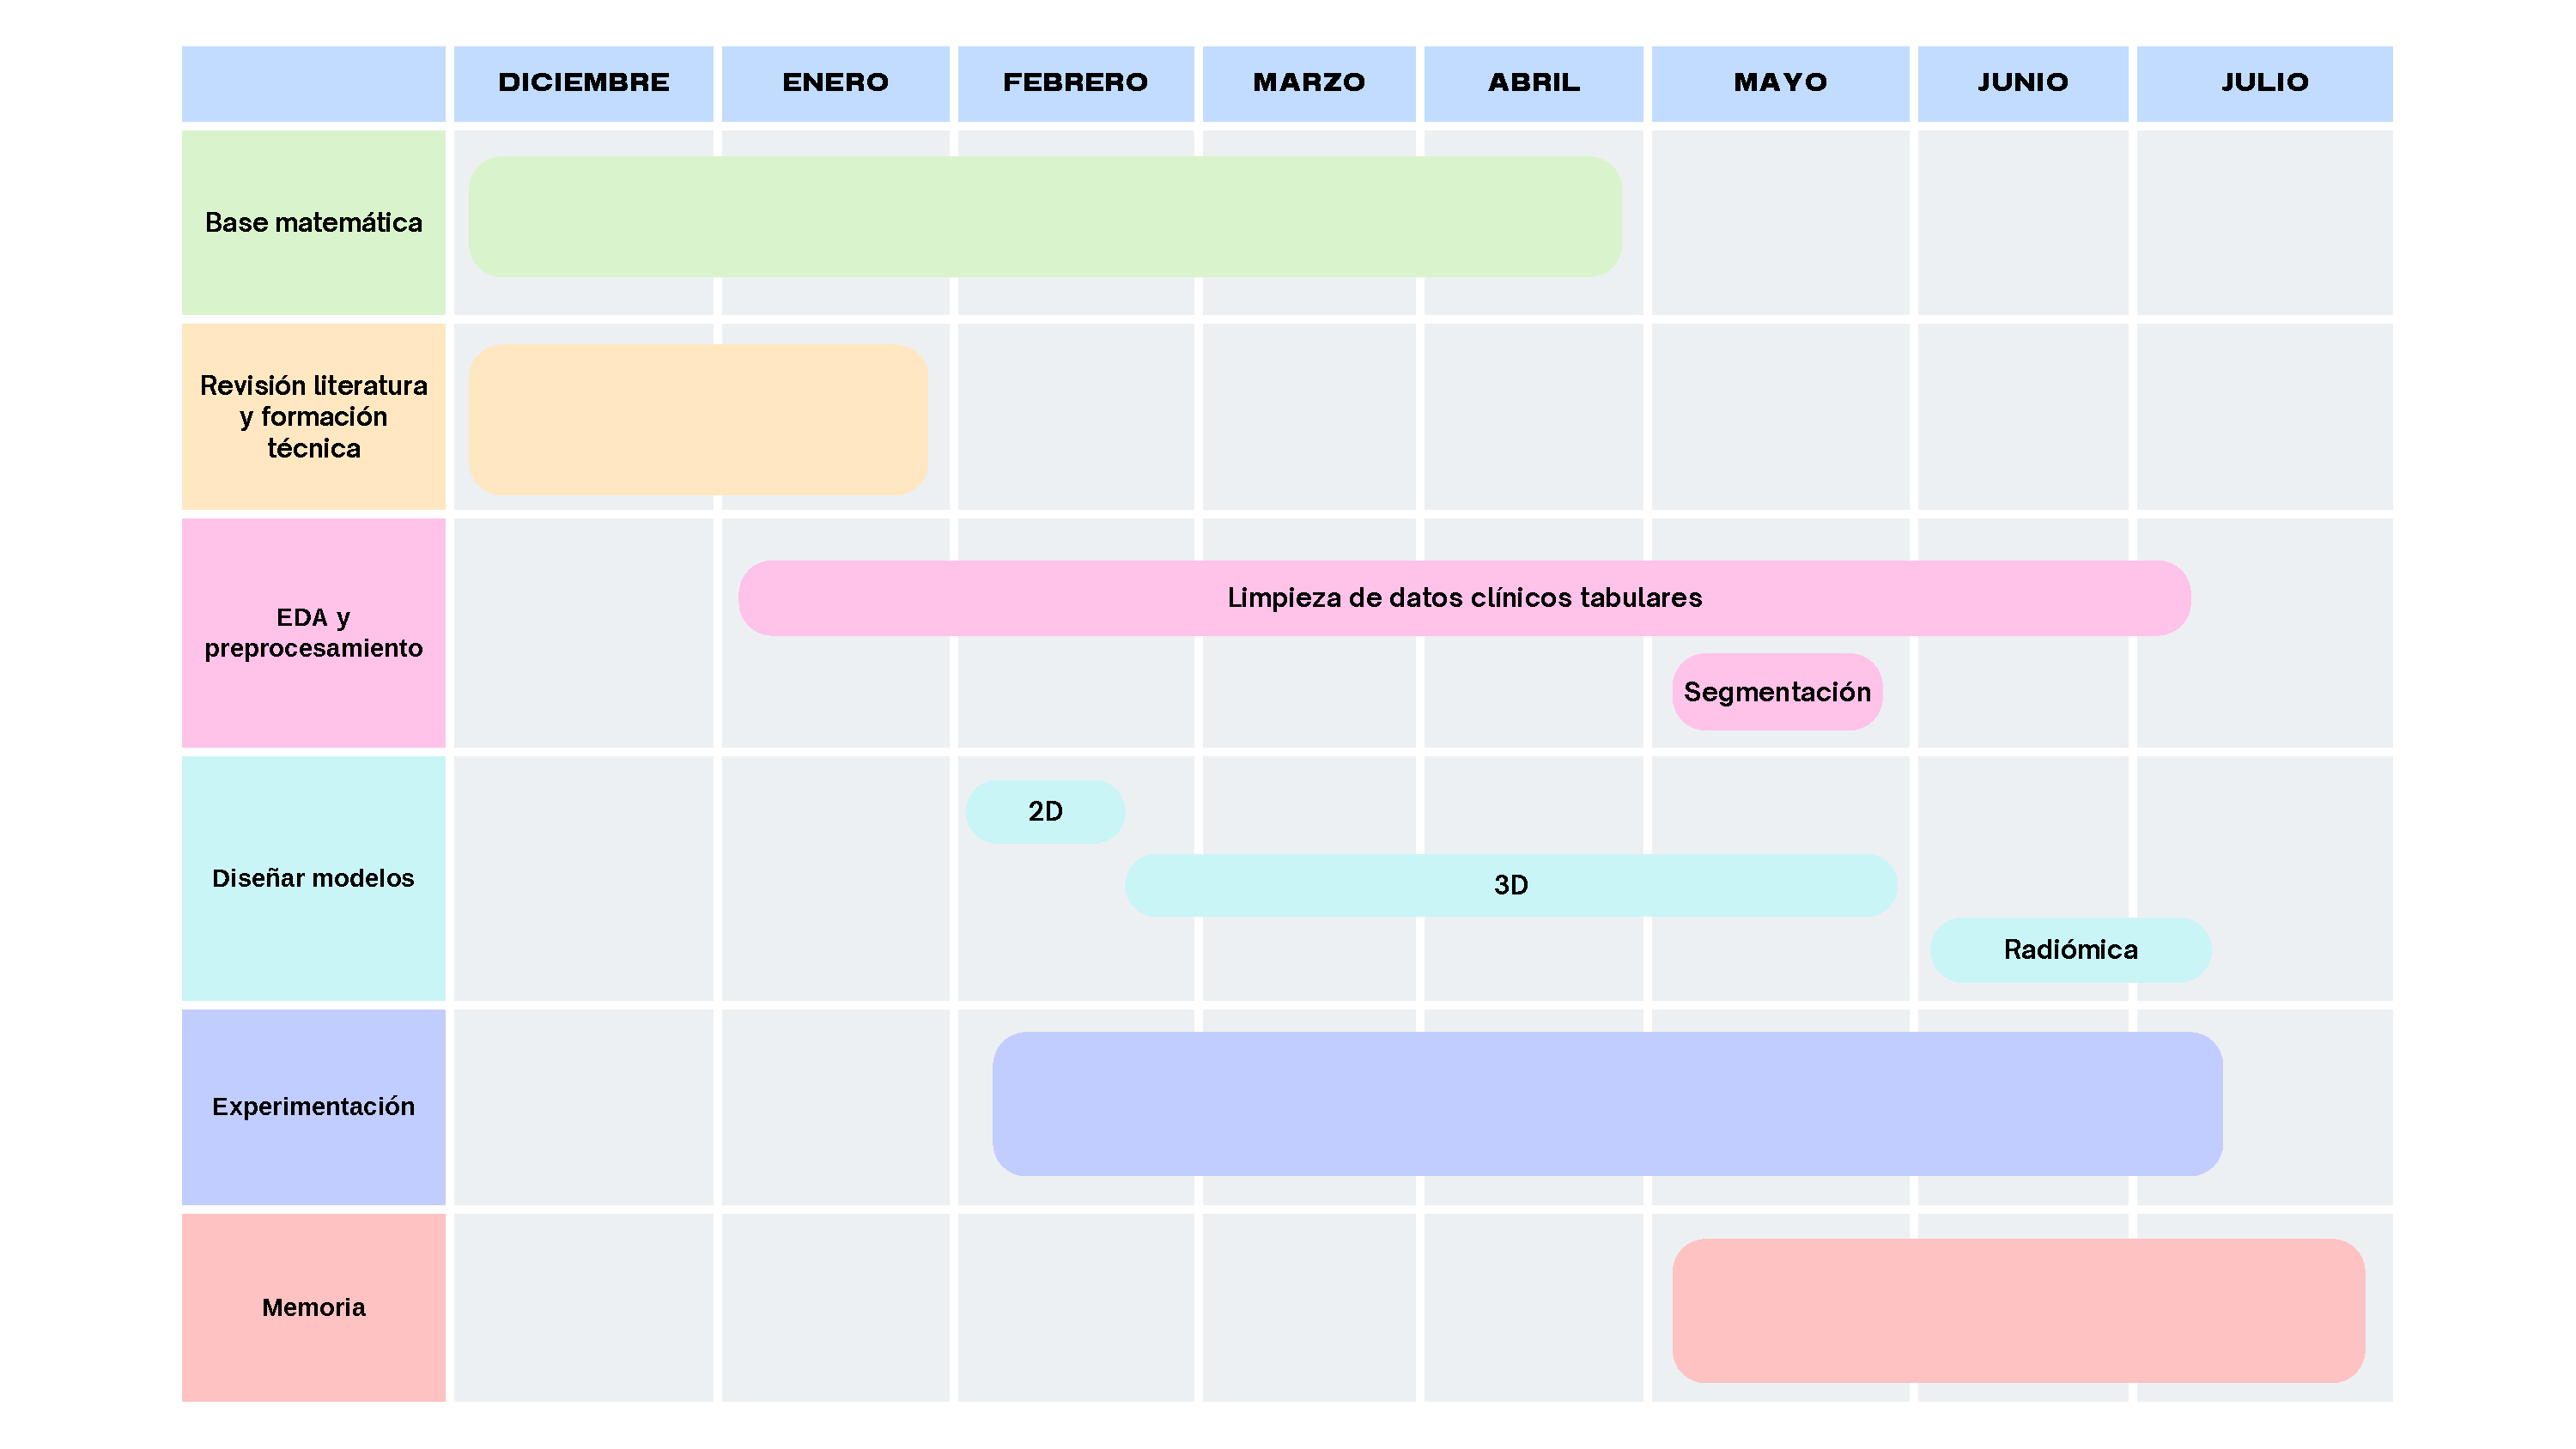
\includegraphics[width=1.1\textwidth]{img/gantt.pdf}
    \caption{Diagrama de Gantt del proyecto}
    \label{fig:gantt_chart}
\end{figure}

\endinput
%--------------------------------------------------------------------
% FIN DEL CAPÍTULO. 
%--------------------------------------------------------------------
